\section{Day night cycle}
Even though the game can be played in non-Euclidean spaces which makes it inherently unrealistic, we decided to add some elements that would make the scenes portrayed in the game feel familiar.
In particular, one property of the real world that we wanted to capture in the game was the daytime cycle.
In the game, the full cycle is 10 minutes long, with 5 minutes long daytime and 5 minutes long nighttime.
We also added transitions between day and night to give the Earth-like experience of sunrise and sunset.
The scene during various times of the day is shown in \autoref{fig:cycle}.

\begin{figure*}[h]
    \centering
    \begin{subfigure}[b]{0.475\textwidth}
        \centering
        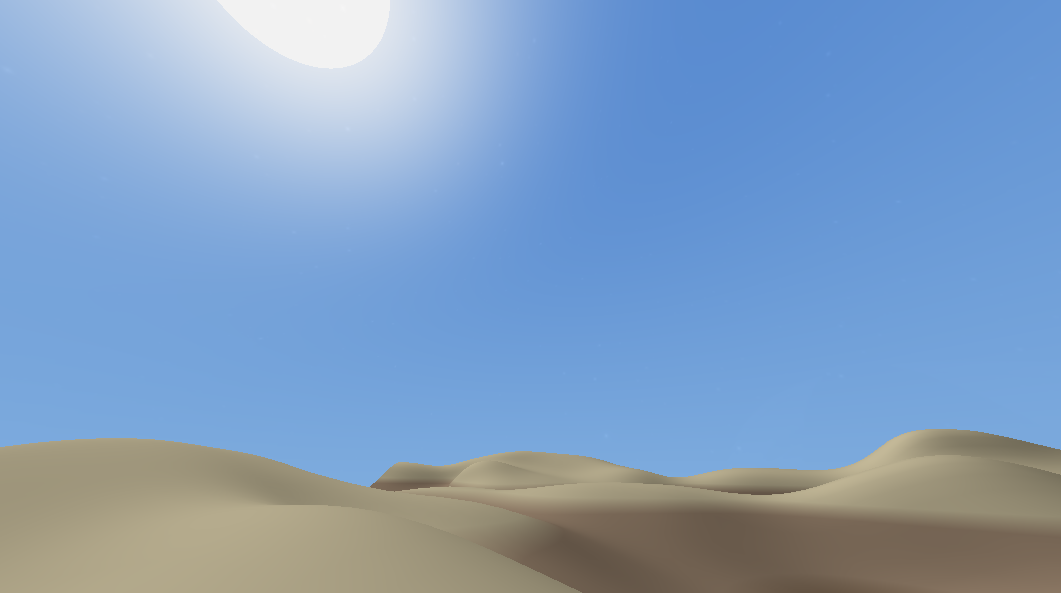
\includegraphics[width=\textwidth]{chapters/theoretical_foundations/sections/day_night_cycle/resources/day.png}
        \caption[]%
        {{\small Day}}
        \label{fig:cycle-day}
    \end{subfigure}
    \hfill
    \begin{subfigure}[b]{0.475\textwidth}
        \centering
        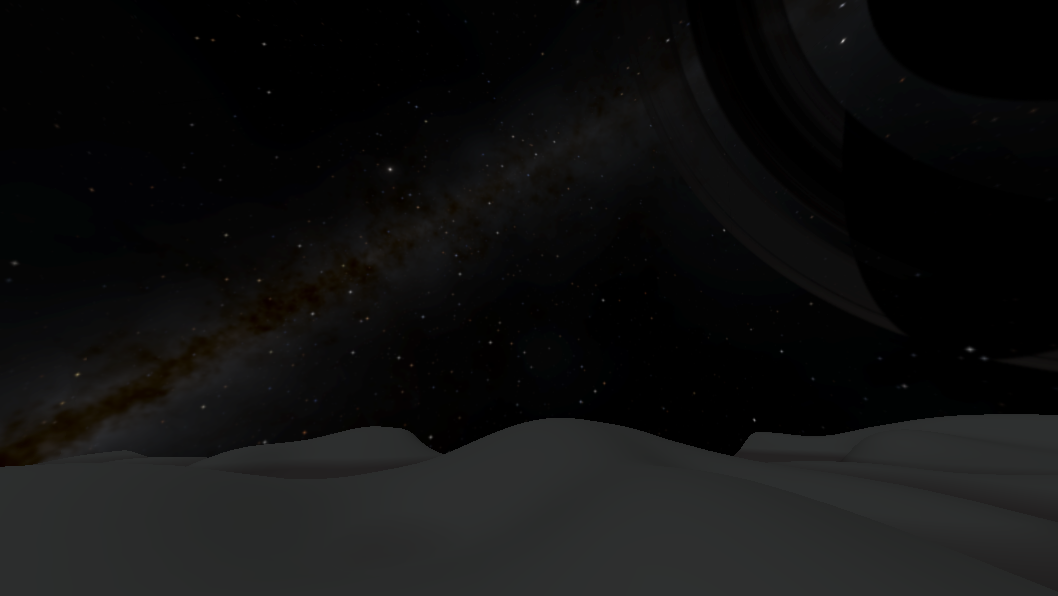
\includegraphics[width=\textwidth]{chapters/theoretical_foundations/sections/day_night_cycle/resources/night.png}
        \caption[]%
        {{\small Night}}
        \label{fig:cycle-night}
    \end{subfigure}
    \vskip\baselineskip
    \begin{subfigure}[b]{0.475\textwidth}
        \centering
        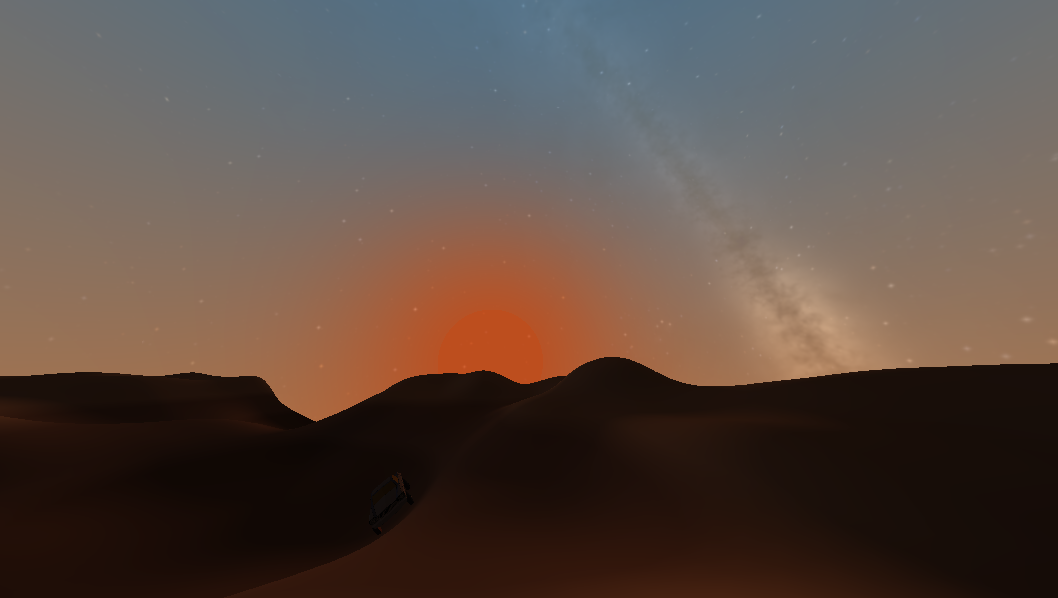
\includegraphics[width=\textwidth]{chapters/theoretical_foundations/sections/day_night_cycle/resources/sunrise.png}
        \caption[]%
        {{\small Sunrise}}
        \label{fig:cycle-sunrise}
    \end{subfigure}
    \hfill
    \begin{subfigure}[b]{0.475\textwidth}
        \centering
        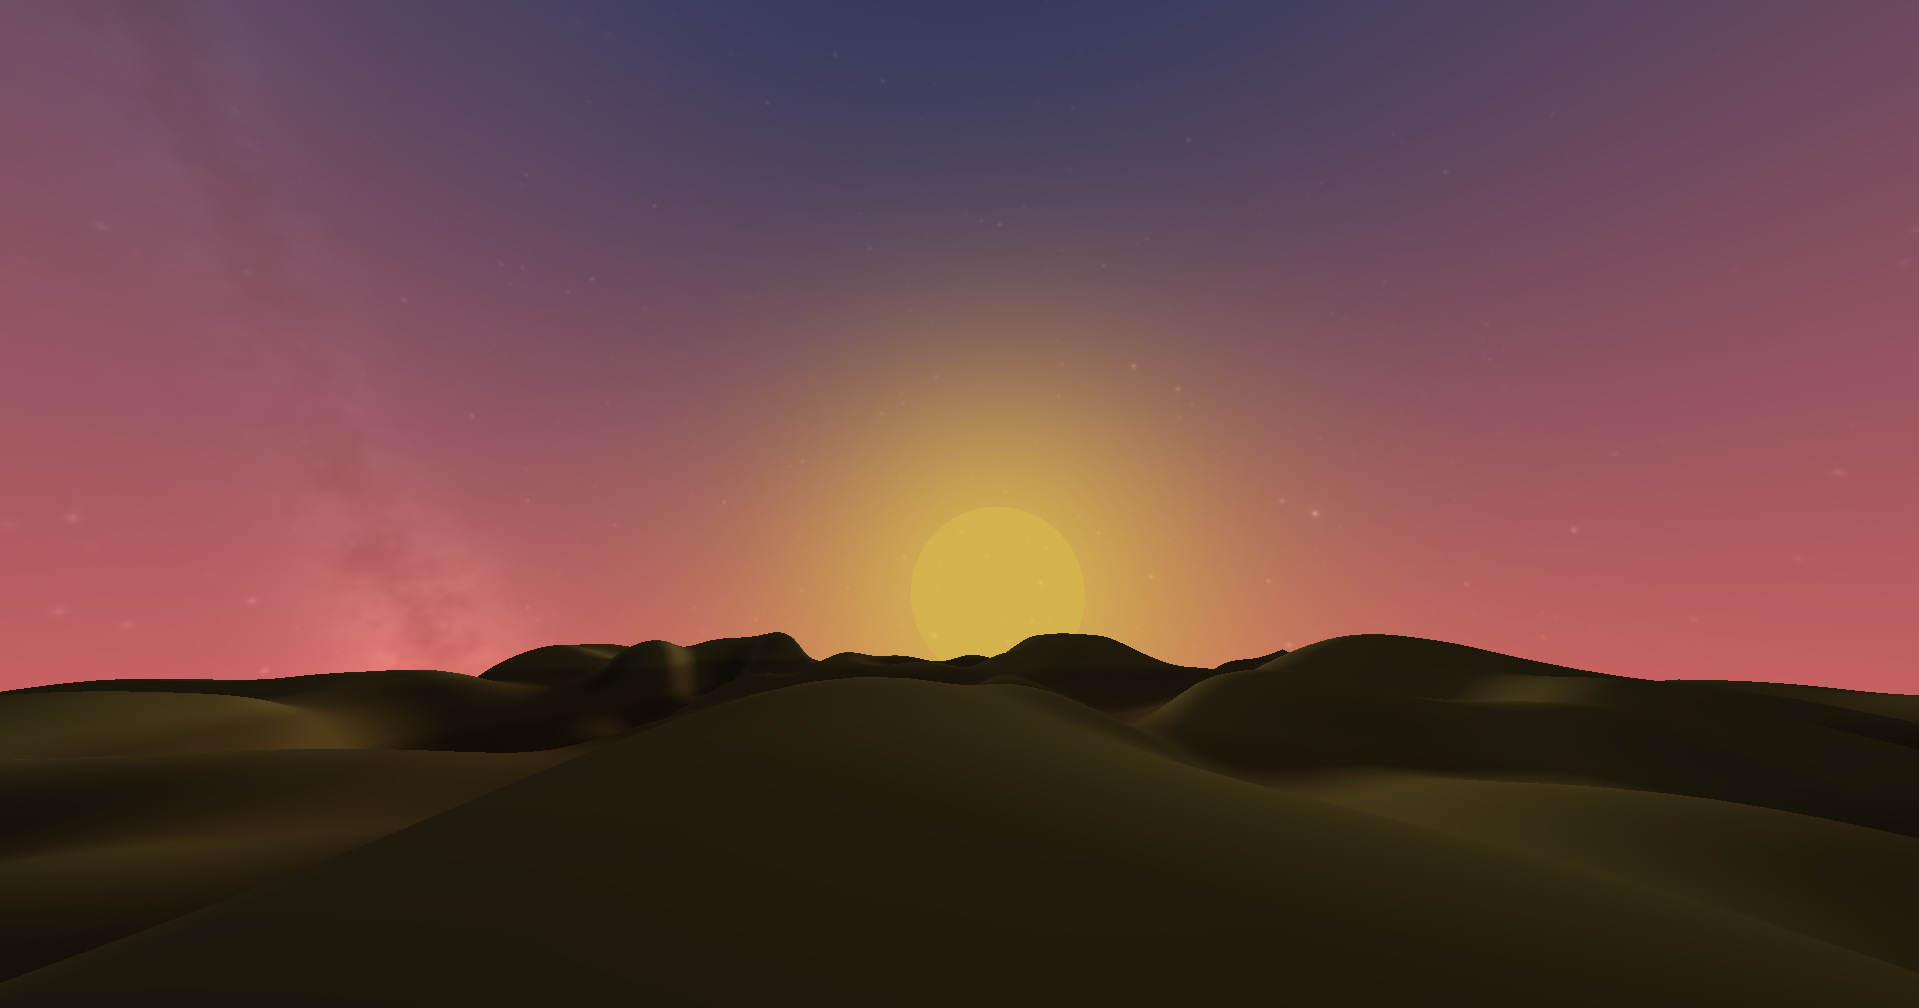
\includegraphics[width=\textwidth]{chapters/theoretical_foundations/sections/day_night_cycle/resources/sunset.png}
        \caption[]%
        {{\small Sunset}}
        \label{fig:cycle-sunset}
    \end{subfigure}
    \caption[]
    {\small Day night cycle in the game}
    \label{fig:cycle}
\end{figure*}

The implementation of the day-night cycle relies on two components: directional lighting (described in \autoref{subsec:directional-lighting}) which corresponds to the light coming from the sun and a \textit{skybox} representing the sky.
Conceptually, a skybox is a cube made out of 6 images, one per each side, that encompasses the scene thus creating an illusion that the world is much bigger than it is in reality.
A skybox can be implemented in OpenGL using a special type of texture, a \textit{cubemap}, i.e. a texture that contains 6 individual 2D textures.
In the game, we're using images of the night sky obtained from an HDR file \url{https://www.reddit.com/r/blender/comments/3ebzwz/free_space_hdrs_1/} using an online utility program \url{https://matheowis.github.io/HDRI-to-CubeMap/}.
The images were then slightly edited by applying Gaussian blur to make the stars appear larger.
The vertices of the cube passed to the vertex shader are transformed using the model, view, and projection matrices.
The model matrix is responsible for rotating the skybox (similarily to how stars appear to move across the night sky as the Earth is rotating).
The view matrix has to be modified so that the skybox doesn't move along with the camera.
The part responsible for translation can be removed from the view matrix by replacing the last row the the view matrix with the vector $ \begin{bmatrix} 0 & 0 & 0 & 1 \end{bmatrix} $ \cite{LearnOpenGL-Cubemaps}.

The day is split into \textit{phases}, each characterized by the color of the sky at the zenith, the sky's color at the horizon, the color of the sun, and \textit{stars' visibility factor}.
In the fragment shader, we determine the color of each fragment.
This is done by first obtaining the zenith and horizon colors by interpolating between the corresponding colors for the previous and the next phase based on the current time.
In the same manner, we obtain the current stars' visibility factor.
Then, we obtain a sky color for a given fragment by interpolating between the zenith and horizon colors based on the height of the fragment\footnote{The "position" of a fragment in this context is given by world space coordinates, normalized so that we're treating the points as located on a sphere (\textit{skydome}). The height is then simply the $y$ coordinate of the fragment's position.}.
The sun's position is given by a vector $s$ that rotates at the same rate as the skybox.
Calculating a dot product $d$ of $s$ with the current fragment's position allows us to easily draw the sun and the sun glare by mixing the sky's color with the sun's color in proportions depending on $d$.
As the last step, we mix the pure-day-time color of the sky with the pure-night-time texture of the stars in proportions given by the stars' visibility factor.

The day-night cycle hasn't been implemented for the spherical space, as the terrain in the spherical space fully "encloses" the scene leaving no way of seeing anything "outside".